\documentclass[12pt,a4paper]{article}
\usepackage{ctex}
\usepackage{listings}
\usepackage{xcolor}
\usepackage{fancyhdr}
\usepackage{graphicx}
\pagestyle{fancy}
\rhead{Mingchen Liu}
\lstset{
    %backgroundcolor=\color{red!50!green!50!blue!50},%代码块背景色为浅灰色
    rulesepcolor= \color{gray}, %代码块边框颜色
    breaklines=true,  %代码过长则换行
    numbers=left, %行号在左侧显示
    numberstyle= \small,%行号字体
    %keywordstyle= \color{red},%关键字颜色
    commentstyle=\color{gray}, %注释颜色
    frame=shadowbox%用方框框住代码块
    }

% Title
\title{《数学建模与最优化》课程作业}
\author{刘铭宸\\软件工程2003班\\U202010783}
\date{\today}
 
\begin{document}

\begin{titlepage}
\maketitle
\end{titlepage}

\tableofcontents

\newpage
\section{最速下降法}
\subsection{方法介绍}
在基本迭代公式
$x_{k+1}=x_k+t_kp_k$中 ,每次迭代搜索方向$p_k$取为
目标函数$f(x)$ 的负梯度方向,即$p_k=-\nabla f(x_k)$,而每次迭代的步长$t_k$
取为最优步长,由此所确定的算法称为最速下降法。
最速下降法是法国数学家
Cauchy于1874年提出的,是求解无约束
最优化问题最早使用的方法之一,也是现代优化方法的基础。
\subsection{迭代步骤}
已知目标函数$f(x)$及其梯度$g(x)$,终止限$\varepsilon$,最速下降法的迭代步骤如下:
\begin{enumerate}
    \item 选定初始点$x_0$,置$k=0$.
    \item 计算$g_k=g(x_k)$.
    \item 若$||g_k||<\varepsilon$,则$x^*=x_k$,输出$x^*$,结束;
    否则令$p_k=-g_k$,由一维搜索求步长$t_k$,使得
    \begin{equation}
        f(x_k+t_kp_k)=min_tf(x_k+tp_k),t>0
    \end{equation}
    \item 令$x_{k+1}=x_k+t_kp_k$,置$k=k+1$,转2.
\end{enumerate}

\subsection{编程实现}
例:用最速下降法求函数$f(x)=2x_1^2+x_2^2$的极小点。设初始点为$x_0=(1,1)^T,\varepsilon = 1/10$.

根据老师关于最速下降法的介绍,编写代码如下:
\begin{lstlisting}[language={python}]
    import numpy as np
    from sympy import *
    import math

    x1, x2, t = symbols('x1, x2, t')
    
    def func():
        return 2*pow(x1, 2) + pow(x2, 2)
    
    def grad(data):
        f = func()
        grad_vec = [diff(f, x1), diff(f, x2)]
        grad = []
        for item in grad_vec:
            grad.append(item.subs(x1, data[0]).subs(x2, data[1]))
        return grad
    
    def grad_len(grad):
        vec_len = math.sqrt(pow(grad[0], 2) + pow(grad[1], 2))
        return vec_len
    
    def zhudian(f):
        t_diff = diff(f)
        t_min = solve(t_diff)
        return t_min
    
    def main(X0, theta):
        f = func()
        grad_vec = grad(X0)
        grad_length = grad_len(grad_vec)
        print("梯度模长",grad_length)
        k = 0
        print("x"+str(k)+"=(",X0[0],",",X0[1],")")
        data_x = [0]
        data_y = [0]
        while grad_length > theta:
            k += 1
            p = -np.array(grad_vec)
            X = np.array(X0) + t*p
            t_func = f.subs(x1, X[0]).subs(x2, X[1])
            t_min = zhudian(t_func)
            X0 = np.array(X0) + t_min*p
            grad_vec = grad(X0)
            grad_length = grad_len(grad_vec)
            print('梯度模长', grad_length)
            print("x"+str(k)+"=(",X0[0],",",X0[1],")")
            data_x.append(X0[0])
            data_y.append(X0[1])
        print("迭代次数:",k)
        
    if __name__ == '__main__':
        main([1, 1], 0.1)

\end{lstlisting}
~\\
计算结果如下图:
\begin{figure}
    \centering
    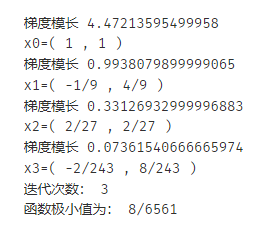
\includegraphics[scale=0.8]{steepest.png}
    \caption{最速下降法结果}
    \label{fig:1}
\end{figure}

    ~\\~\\~\\~\\~\\~\\~\\~\\~\\~\\
    \subsection{结果分析}

    结果显示,最速下降法总共迭代了3次,
    最终求得函数极小值为$8/6561$,
    此时自变量$x$为$(-2/243,8/243)^T$。
    最终迭代误差为0.07361540666665974,
    显然达到了实验预设误差要求。

\section{牛顿法}
\subsection{方法介绍}
Newton法的基本思想是利用目标函数$f(x)$在迭代点$x_k$处的二次
Taylor多项式作为二次函数,并用这个二次函数的极小点序列去
逼近目标函数的极小点。
\subsection{迭代步骤}
已知目标函数$f(x)$,终止限$\varepsilon$,Newton法的迭代步骤如下:
\begin{enumerate}
    \item 选定初始点$x_0$,置$k=0$.
    \item 计算$g_k=\nabla f(x_k)$.
    \item 若$||g_k||<\varepsilon$,则$x^*=x_k$,结束;
    否则计算$G_k=G(x_k)=\nabla ^2f(x_k)$.
    \item 由方程$G_kp_k=-g_k$解出$p_k$.
    \item 令$x_{k+1}=x_k+p_k$,置$k=k+1$,转2.
\end{enumerate}

\subsection{编程实现}
例:试用 Newton 法求函数$f(x_1,x_2)=x_1^2+4x_2^2$的极小点,
初始点为$x_0=(1,1)^T$,精度要求$10^{-6}$.
根据老师关于Newton法的介绍,编写代码如下:
\begin{lstlisting}[language={python}]
    import numpy as np

    def fun(x):     
        return x[0] ** 2 + 4 * x[1] ** 2

    def gfun(x):
        return np.array([2 * x[0], 8 * x[1]], dtype=float)

    def Gfun(x):
        return np.array([[2, 0], [0, 8]], dtype=float)

    def Newton(x0, eps=10 ** (-6)):
        xk, count = x0, 0
        print("梯度模长", np.linalg.norm(gfun(xk)))
        while np.linalg.norm(gfun(xk)) > eps:
            count += 1
            gk = gfun(xk)
            Gk = Gfun(xk)
            dk = -np.linalg.inv(Gk) @ gk
            xk = xk + dk
            print("迭代次数:",count)
            print("梯度模长", np.linalg.norm(gfun(xk)))
        return xk, count

    if __name__ == '__main__':
        x0 = np.array([[1], [1]])
        x = Newton(x0)
        print('极小值点:', x[0].T, '极小值:', fun(x[0]))
\end{lstlisting}
~\\
计算结果如下图:
~\\~\\~\\~\\~\\~\\~\\~\\~\\~\\~\\~\\
\begin{figure}
    \centering
    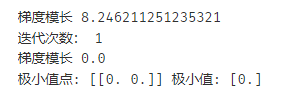
\includegraphics[scale=1.0]{Newton.png}
    \caption{Newton法结果}
    \label{fig:2}
\end{figure}
~\\~\\~\\~\\
\subsection{结果分析}

结果显示,Newton法总共迭代了1次,
最终求得函数极小值为0,
极小值点$x$为$(0,0)^T$,
最终迭代误差为0,得到了精确解,
显然达到了实验预设误差要求。

\section{DFP方法}
\subsection{方法介绍}
DFP方法是最早的拟牛顿法,该算法的核心是:通过 迭代的方法,对$H_{k+1}^{-1}$做近似,迭代格式为$D_{k+1}=D_k+\nabla D_k,k=1,2,\dots$

\subsection{迭代步骤}
\begin{figure}
    \centering
    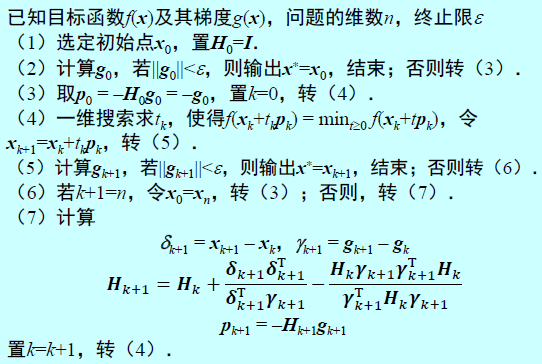
\includegraphics[scale=0.6]{DFP.png}
    \caption{DFP方法迭代步骤}
    \label{fig:3}
\end{figure}
~\\~\\~\\~\\~\\~\\~\\
\subsection{编程实现}
例:用DFP方法求函数$f(x_1,x_2)=x_1^2+4x_2^2$的极小点。
初始点为$x_0=(1,1)^T$,精度要求$10^{-6}$.

根据老师关于DFP方法的介绍,编写代码如下:
\begin{lstlisting}[language={python}]
    import numpy as np
    import sympy as sp
    def jacobian(f,x):
        a,b=np.shape(x)
        x1,x2=sp.symbols('x1 x2')
        x3=[x1,x2]
        df=np.array([[0.00000],[0.00000]])
        for i in range(a):
            df[i,0]=sp.diff(f,x3[i]).subs({x1:x[0][0],x2:x[1][0]})
        return df

    def hesse(f,x):
        a,b=np.shape(x)
        x1,x2=sp.symbols('x1 x2')
        x3=[x1,x2]
        G=np.zeros((a,a))
        for i in range(a):
            for j in range(a):
                G[i,j]=sp.diff(f,x3[i],x3[j]).subs({x1:x[0][0],x2:x[1][0]})
        return G
        
    def dfp_newton(f, x, iters):
        a = 1
        H = np.eye(2)
        G=hesse(f,x)
        epsilon = 1e-6
        for i in range(1, iters):
            g = jacobian(f, x) 
            if i == 1:
                print("||g0||=",np.linalg.norm(g))
            else:
                print("||g(k+1)||=",np.linalg.norm(g))
            if np.linalg.norm(g) < epsilon:
                xbest=[]
                for a in x:
                    xbest.append(a[0])
                break
            d= -np.dot(H,g)
            a=-(np.dot(g.T,d)/np.dot(d.T,np.dot(G,d)))
            x_new = x +a*d
            print("第 %d 次迭代"%i)  
            print("x=",x_new)
            g_new = jacobian(f, x_new)
            y = g_new - g
            s = x_new - x
            H=H+np.dot(s,s.T)/np.dot(s.T,y)-np.dot(H,np.dot(y,np.dot(y.T,H)))/np.dot(y.T,np.dot(H,y))
            G=hesse(f,x_new)
            x = x_new 
        return xbest
        
    x1,x2=sp.symbols('x1 x2')
    x=np.array([[1],[1]])
    f=x1**2+4*x2**2
    X = dfp_newton(f,x,20)
    print("极小值为:",X[0]**2+4*X[1]**2)
\end{lstlisting}
~\\
计算结果如下图:
~\\~\\~\\~\\~\\~\\
\begin{figure}
    \centering
    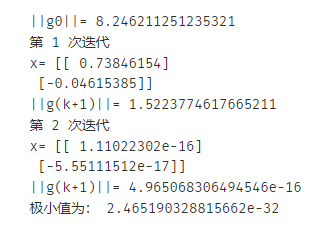
\includegraphics[scale=1.0]{DFP_2.png}
    \caption{DFP方法结果}
    \label{fig:3}
\end{figure}
~\\~\\~\\~\\~\\~\\~\\~\\
\subsection{结果分析}

结果显示,DFP方法总共迭代了2次,
最终求得函数的极小值为$2.465\times 10^{-32}$,
此时自变量$x$为$(1.110\times 10^{-16}, -5.551\times 10^{-17})^T$,
最终迭代误差为$4.965\times 10^{-16}$,
显然达到了实验预设误差要求。

~\\~\\~\\
感谢卢力老师一学期的教学!
\end{document} 